\documentclass[12pt]{article}
\usepackage{fullpage}
\usepackage{textcomp}
\usepackage{graphicx}
\usepackage{amssymb}
\usepackage{amsmath}
\usepackage{float}

\author{
Jack Hedlund-Fay\\hedlu131@umn.edu
}

\title {Building a Better Mouse \\
\large On Training an Agent to Solve Mazes}

\begin{document}

\maketitle

\renewcommand{\theenumii}{\arabic{enumii}}
\renewcommand{\labelenumii}{\theenumii)}
\renewcommand{\theenumiii}{\arabic{enumiii}}
\renewcommand{\labelenumiii}{\theenumiii.}

\section{Abstract}

\section{Introduction}

\hspace*{\parindent} In \textit{Using Search Algorithms for Better Walking Direction}, I investigated the history, interest, and practical applications of shortest-path algorithms such as Dijkstra's algorithm or A* and used those algorithms to develop a program that could, given a source and a destination point on a binary map, find the shortest path between those points. One useful application of the shortest path algorithms is their ability to solve mazes. Given a starting node and a destination, algorithms such as Dijkstra's and A* are guaranteed to find the shortest path through the maze. Upon reflection, however, these algorithms are not practically useful for solving mazes because while one is in a maze they cannot know the layout of the maze and they do not know where the destination is until they are upon it. To the end of finding a path when the program is nonomniscient, different approach must be used. The maze solving algorithms are methods used for the solving of mazes when the agent involved has no prior knowledge of the maze. The trivial method for maze solving, following paths and making random choices when arriving at a junction, is called the random mouse algorithm after Robert Tryon's 1940 experiment on rats in mazes.

\hspace*{\parindent} In 1940, Tryon conducted a psychological experiment on rats in which, over several generations, he separated "maze-bright" rats\textemdash rats that performed well on a novel maze\textemdash from "maze-dull" rats, bred them together and cross-fostered them. This experiment was conducted to determine whether or not genetic differences produced individual behavioral variations and found that the "bright" rats in the experiment, by the seventh generation, performed significantly better on novel mazes than the "dull" rats. Though there were problems with how the experiment was conducted, as later research found, the idea of the experiment is an interesting one and one which connects to many artificial intelligence concepts. In this experiment, I intend to recreate Tryon's rat experiment, only instead of using actual rats I intend to create a "rat" agent and investigate whether or not I can, by posing maze-solving as an optimization problem, approach known maze-solving algorithms that are faster than random mouse, by using the genetic algorithms and selecting rat agents that are more fit to solve mazes over consecutive generations.

\hspace*{\parindent} The genetic and evolutionary algorithms are approaches to optimization problems that were pioneered in the 1950s and 60s by computer scientists including John Henry Holland. These algorithms draw inspiration from Charles Darwin's theory of evolution and biological concepts such as mutation, crossover, and selection as a path to generating high-quality optimization solutions. The original genetic algorithms used strings of binary values where each binary value in the string represents a single gene, a single string of binary values represents a chromosome, and all of the strings of chromosomes constitute a population. For a genetic algorithm to work a fitness function must be able to be defined; that is, a function to determine how fit an individual is compared to the other individuals in the population. The selection phase of the algorithm uses the fitness scores calculated and chooses the fittest individuals to be chosen for reproduction. Offspring are generated by taking the fittest individuals selected and randomly combining their genes into a new individual. In the binary string example this can be done by randomly selecting an index in the string and switching the values between two parent individuals for all indices before the randomly chosen index. Additionally, with a random low probability certain genes will be mutated. In the binary string example this means after selection and crossover at a random low probability some of the genes will be changed from a 1 to a 0 or vice versa. This algorithm runs to convergence: a point after which the offspring are cease to be significantly different from the previous generation. While Holland primarily worked with strings of bits, trees, lists, or other objects can be used in the genetic algorithm as long as the key genetic operators (initialization, mutation, crossover, comparison) can be defined for the chosen representation. In order to choose what information will constitute a chromosome in my rat agent population and how the genetic operators for these chromosomes will be defined I must first look at the existing maze-solving algorithms and what the key information is that is involved in these algorithms.

\hspace*{\parindent} The simplest method to solving a maze is the random mouse algorithm. In this method the agent follows along the current passage until they reach a junction and chooses a random direction at every junction. The next simplest maze-solving method is the wall follower method or the left-hand rule. Given a simply connected maze; that is, one where every wall in the maze is connected together, one is guaranteed to always be able to eventually find their way out by keeping their left (or right) hand in contact with a wall of the maze. The trouble with this approach obviously comes from scenarios where the maze is not simply connected in which case the agent in the maze must be able to observe when their tracing the wall brings them back to a point in the maze that they have already been to once before in whcih case they should switch to a different wall not yet followed and try again. The Pledge algorithm (named for Jon Pledge), goes a step further and allows for the solving of any finite two-dimensional maze as long as the agent navigating the maze know what direction they are facing at any given time (i.e. if they have a compass). The Pledge algorithm starts by choosing a direction to follow and will follow that direction unless following that direction is impossible in which case wall-following takes over and the number of turns made while wall-following is counted. Wall-following only stops when the the agent is both heading in their chosen direction and the sum of the angles of the turns they've made equals zero. This approach is better than wall-following but only works for mazes where the exit is on an outside edge of the maze. It cannot guarantee being able to reach an arbitrary end from an arbitrary beginning within the maze though. Lastly, I will consider Tr\'{e}maux's algorithm. Tr\'{e}maux's algorithm can solve any two-dimensional maze. This algorithm works by keeping track of where the agent has been. When the agent reaches a new junction, like the random mouse, they choose a random new direction and follow that direction, when the agent reaches a dead-end they backtrack the way they came, when an agent following a new path reaches a junction they've been to before they treat it as a dead end and go back the way they came, when the agent following a path they've been down before reaches a junction they take a new passage if one is available or else follow a passage they've been down only once before ignoring any passages they've been down twice before. If the maze has a solution there will be a path that has been traversed exactly once leading from the start to the end and if there are no solutions to the maze all paths in the maze will have been traversed exactly twice. These algorithms, taken together, will not only provide me with benchmarks that I can compare my rat agents to but also inform me of what particular bits of information my rat agents should have access to that they can then factor in to their maze solving approach.

\section{Background}

\hspace*{\parindent} The subject of of using genetic algorithms to as an approach to optimizing the maze-solving problem has been done before. In their 2018 paper, \textit{Maze Navigation via Genetic Optimization}, Webb et. al. investigated the time to convergence on increasingly complex sets of mazes comparing tradtional genetic algorithms that only converged over time from a purely evolutionary approach to genetic algorithms provided rules that were domain-specific to the maze-solving problem. In their approach, each cell of the maze was represented as an encoded string of length four where each of the values in the string represented one of the cardinal directions and whether moving in that direction was a legal move or not; that is, whether or not there was a wall in that direction at that particualar cell in the maze. In their experiment they used distance as their objective function and weighed it as: 

\begin{center}
 $f(x)_{Weighted} = W1 - W2 * (\sqrt{((x_{actual}-x_{final})+(y_{actual}-y_{final})^2)}-W3*(npath-C))$ 
\end{center}

All of the sequences of moves that resulted in a path from the beginning of the maze to the end of the maze were kept, bred together, and mutated where basically the crossover of genes between the parents was done as the recombination of moves through the maze. Of the offspring produced, only those that made legal moves through the maze were kept and the process was repeated keeping only the offsrpring at each iteration that reduced the weighted objective function. Interestingly, the didn't require the sequence of moves to be able to solve the maze, only that the sequence of moves was legal within the maze. In this way, rather than their experiment being one which tested consecutive generations of maze solvers and whether through optimization they could get through the maze faster theirs was an experiment which tested consecutive generation of maze travelers and whether they could make it farther through the maze based solely on the information of their predecessors. 

\hspace*{\parindent} The process that Webb et. al. used in their genetic optimization approach via embedded rules, interestingly, approaches a maze-solving algorithm not yet discussed. The dead-end filling algorithm is yet another algorithm for solving mazes which fills in cells starting from the dead ends until only the correct path(s) through the maze remain. This approach does not work for the rat agent because it requires knowledge about the maze as a whole. However, in Webb et. al.'s experiment, since they were using the genetric algorithm only on a single maze at a time, whenever a dead end was discovered that particular cell would have a wall added such that it became a box. In this way, subsequent generation would essentially be learning which paths led to dead ends and would stop traveling down those paths as generations passed. In this way it is as though, in addition to information about legal moves, the subsequent generations of maze travellers in Webb et. al.'s experiment were being passed information from their predecessors about which paths they shouldn't travel down. When the traditional genetic optimization approach was compared against the genetic optimization approach with embedded rules for the same 10x10 maze, the embedded rules maze solving was able to solve the maze in the time it took the traditional genetic algorithm to get through only about half of the maze. The experimenter observed that, while the traditional genetic algorithm would have eventually converged to a solution to the maze, such a solution would require and unnacceptably large number of generations for their purporses.

\hspace*{\parindent} The article, \textit{Solving A 2D Maze Game Using a Genetic Algorithm and A* Search - Part 2}, by Tony Truong goes into more detail about the specifics of how to implement a genetic algorithm to solve a maze. Firstly, the article covers the key components of a genetic algorithm approach to optimization and each of those components corresponds to in the maze-solving optimization problem. The article gives the key components of a genetic algorithm approach as a large, random initial population, some objective fitness function to define how close an individual in the population is to the desired solution, some way to select only the fittest members of the population, some way to "mate" and crossover the fittest indiviudals such that the offspring have similar genes to their parents, and a degree of mutation to prevent early converence.  The indivudals in Truong's representation for the maze solving problem were an array of moves with a maximum upper move limit. That is; each array represents a number of legal moves within the maze up to the maximum number of moves allowed or until the solution cell is reached. Because the maze problem is on the cartesian plane, Truong chose to represent the fitness function as Manhattan distance:

\begin{center}
$d = |x_2 - x_1| + |y_2 - y_1|$
\end{center}

Notably, rather than informing the algorithm as to which directions were legal moves or not from the beginning, Truong allowed for moves that would cause the agent involved to walk into a wall and imposed an additional penalty on offspring which produced solutions that involved them walking into walls. In this way the genetic algorithm optimization appraoch can, at least, rapidly approach the random mouse algorithm in terms of the quality of solutions being found by the offspring. In order for a maze-solving agent to reach the level of random mouse they must, at least, know to make a legal move down a corridor and not simply make a random move at every point in the maze. Interestingly, Truong's approach had the potential to return "solutions" to the maze that did not solve the maze. This is because, rather than producing a population that found the solution to the maze, he produced a population that found paths that came close to where the solution actually was. This resulted in some of the solutions returned including paths that lead to dead ends where the cell of the dead end happened to be close to the where the actual exit was. This is important because it indicates the limitations of using distance to the finish as the fitness function for maze solving, rather one must consider an approach that uses the minimum number of legal moves remaining to reach the end goal as the fitness function.

\section{Problem}

\hspace*{\parindent} My version of this problem differs in a critical way from either Webb et. al.'s experiment or Truong's article in that, rather than being concerned with the optimality of the maze solution by my rat agents (though that will be a consideration), I would like my rat agents to be able to learn a consistent methodolgy by which they could solve any maze they are put into. Because this is my goal, I have carefully considered what information must be made available to my initial rat population in order for them to reach the maze-solving algorithms that I intend to compare the performance against. 

All of my rats will have an effective "vision" of 1 and the ability to know where they have been. However, the initial population of rats will not have any specific way to interpret this available information. 

\begin{figure}[H]
	\centering
	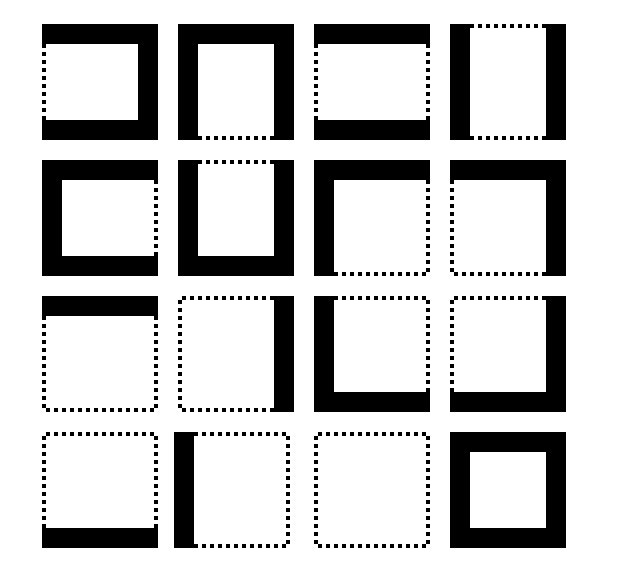
\includegraphics[width=0.4\linewidth]{maze_points.png}
	\caption {The sixteen possible wall arrangements in a 2D grid maze. The sixeenth possibility can be ignored as there is no way in or out of such a tile.}
\end{figure}

The genes, in my problem design, will be key,value pairs in a dictionary representing how the indivdual weighs their options based on their knowledge the tiles adjacent to them. Specifically there will 16 key,value pairs in one individual. Four representing how to weigh the choices in a situation were a particular adjacent cell is inaccessible (there's a wall in the way). With these genes I hope to quickly be able to eliminate all offspring from the population that attempt to walk into walls. Four will represent how to weigh options where there are novel paths; that is, how to weigh the options if one or more of the adjacent cells has not been visited before. The last eight values will represent the weights for paths that the rat has visited only once before or two or more times before. These will hopefully allow me to eliminate from the population those rat agents which would unnecessarily double back or make redundant moves within the maze. With these speifications I believe that my rats can surpass the benchmark of random mouse algorithm. At the very least by knowing not to travel down paths they've been down before, the rats can do slightly better than random at every junction. For each of the mazes in my set, however, I will not only be comparing the genetic rats against a benchmark of rat agents programmed to follow the random mouse algorithm, they will also be compared against the benchmark of rat agents programmed to follow Tr\'{e}maux's algorithm.

\hspace*{\parindent} To the end of being able to have the rats understand where they have already been. In addition to their genetic rules divtionary they will also maintain a "mental" matrix representing the maze where the size of the matrix will match the size of the maze and they will know where a specific tile is within the maze so as to update those values as they travel. 

 \hspace*{\parindent} I hypothesize, based on my knowledge of natural selection models, that the progress of my rat agents will be sigmoidal; that is, the rats will start off slow (since all of the agents will initially only move through the maze randomly) but once mutation sets in and the rat agents learn not to bump into walls and not to move redundantly, I expect the quality of their solutions to rapidly increase until it plateau's off again at roughly the same level as the random mouse algorithm rat agents. Depending on how the experiment proceeds, I may try to add an additional four genes where the key,value pairs would represent paths that have been traversed exactly once versus paths that have been traversed twice or more toward the end of seeing if the genetic rat agents would converge on the Tr\'{e}maux's algorithm solution.

\hspace*{\parindent} To summarize, I will be performing this experiment on a set of genetric rat agents. The rat agents will be allowed to move through the maze until the either reach the solution or hit a maximum number of moves at which point the indivudals in the population that either solved the maze in the fewest number of moves or who have the fewest remaining moves left before they would reach the solution will be selected for breeding. Further, by making a maze for which the path to the solution is complex, I can hopefully ensure that, even though I won't be using novel mazes for each generation (like in Tryon's experiment), the weights learned by the genetic algorithm will represent general maze-solving solutions.

\section{Experiment}

\hspace*{\parindent}  To the end of being able to find a general maze-solving solution, I generated many mazes and chose, for my maze, one that wouldn't cause anomalous weights; that is, there are no easy straight-line or diagonal paths through this maze.

\begin{figure}[H]
	\centering
	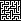
\includegraphics[width=0.4\linewidth]{1.png}
	\caption {The maze I chose for the experiment}
\end{figure}

The first step I took in developing the program was to create a Rat class in python that had the specific attributes of a rat agent that I described in the problem statement. One important detail that I found in developing the rat class was that the dictionary of key,value pairs representing the types of adjacent cells and their associated weights had to be an Ordered Dictionary so that when I was crossing over the rules from parent rats, rule order was preserved. Beyond that, using numpy arrays I was easily able to make a "memory" matrix that represented the rat agent's memory of where they have/have not explored yet in the maze.

The rules ordered dictionary took on this form:

\begin{verbatim}
    rules = [('Nx', 1.0), ('Sx', 1.0), ('Ex',1.0), ('Wx',1.0),
                      ('N0',1.0), ('S0',1.0), ('E0',1.0), ('W0',1.0),
                      ('N1',1.0), ('S1',1.0), ('E1',1.0), ('W1',1.0),
                      ('N+',1.0), ('S+',1.0), ('E+',1.0), ('W+',1.0)]
\end{verbatim}

where Direction+x represents a wall; a direction that the rat cannot travel, Direction+0 represents a novel path, Direction+1 represents a direction the rat has already travelled down (but only once), and Direction++ represents those paths that the rat has already been down twice or more.

The second step was to describe a maze running function. In particular, based on where in the maze the rat currently was I had to provide what the choices were for the rat in each of the four cardinal direction and have it use random number generation to choose among the option available to it weighted on the ordered dictionary of internal rules that particular rat maintained. This turned out to be fairly lengthy to write, but easy enough to get to work correctly. A simple while loop goes through the rat's choices at each cell as it continues its journey through the maze up until the point that it either reaches the solution or runs out of moves.

Once that was done and had a representation of both an initial randomized rat and a maze for it to run through I had to implement the different genetic operators. For selection I implemented a BFS algorithm that could, from any cell in the maze, find the shortest distance in number of cells to the solution square. I originally intended to use both the number of remaining moves and for a particular rat to the solution and the number of moves the rat took to reach a solution once it reached a soution to select for fitness but once I realized that both of these numbers would be decreasing as the fitness of the rats in the popuation increased, I chose to use as the fitness function to select on the sum of both the number of moves the rat took and the minimum number of moves remaining before the rat would reach the solution square. At each generation I would take, from my population of 500 rats, the 20 who were the most fit based on this fitness function.

\begin{verbatim}
def select(rats, scores):
    selected = []
    fitness = [x[2] for x in scores]
    results = list(zip(rats, fitness))
    while len(selected) < NUM_SELECTED:
        selected.append(min(results, key = lambda t:t[1]))
        results.remove(min(results, key = lambda t:t[1]))

    return selected
\end{verbatim}

For crossover, I took a pair of parents randomly seclected from the selected rats and combined their rules by choosing an index within the rules ordered dictionary and making all the rules to one side of that index the first parent's and all the rules to the other the other's. For mutation, I changed the value of one gene in the rule dictionary at random by a float interval between 5 and -5. By changing only one gene at a time in the offspring I hoped to ensure that whatever changes were made it was clear that the change in that particular gene positively affected the result. It's like in a science experiment, if you change alll or several of the variables at once it muddies which of those changes was the one which affected the experiment. While I was developing this program, this approach to mutation did, in fact, seem to work better than allowing all the genes to change randomly slightly in terms of avoiding premature convergence.

\begin{verbatim}
def crossover(d1, d2):
    r_idx = random.randint(0, 15)

    child_rules = []

    items1 = list(d1.items())
    items2 = list(d2.items())

    for idx in range(0,r_idx) :
        child_rules.append(items1[idx])
    for idx in range(r_idx, 16):
        child_rules.append(items2[idx])
    child_rules = MyOD(child_rules)

    return child_rules

def mutate(d):
    i = random.randint(0,(len(d)))
    d.update_pos(i, random.random() * MUTATION_FACTOR * random.randint(-1,1))

    return d
\end{verbatim}

Toward the end of preventing premature convergence I had to try to make informed decisions about what I set the global variables for the program to. In particular, I chose to be rather lenient with the maximum number of moves that the rat could make as it travelled through the maze. Since the decision to allow the rat to know the titles that it ha been to both once and twice or more was informed by the details of how  Tr\'{e}maux's algorithm solves mazes I had to the maximum number of moves to be at least somewhat in excess of the worse-case scenario for  Tr\'{e}maux's or random mouse.In a worst-case scenario, an algorithm like  Tr\'{e}maux's may nearly explore every path in the maze twice (if it can't find the solution early). If I didn't permit the rat to stay in the maze long enough to learn the benefits or lack there of of traversing redundant paths, I couldn't hope for the latter variables in the rules to have any meaningful impact.

\section{Results}

\section{Analysis}

\section{Conclusion}

\section{Bibliography}

\end {document}